%%%%%%%%%%%%%%%%%%%%%%%%%%%%%%%%%%%%%%%%%
% Lachaise Assignment; % LaTeX Template
% Version 1.0 (26/6/2018); 
%% This template originates from: % http://www.LaTeXTemplates.com
%% Authors:% Marion Lachaise & François Févotte % Vel (vel@LaTeXTemplates.com)
%% License: % CC BY-NC-SA 3.0 (http://creativecommons.org/licenses/by-nc-sa/3.0/)
% 
%%%%%%%%%%%%%%%%%%%%%%%%%%%%%%%%%%%%%%%%%
%----------------------------------------------------------------------------------------
%	PACKAGES AND OTHER DOCUMENT CONFIGURATIONS
%----------------------------------------------------------------------------------------

\documentclass{article}

%%%%%%%%%%%%%%%%%%%%%%%%%%%%%%%%%%%%%%%%%
% Lachaise Assignment
% Structure Specification File
% Version 1.0 (26/6/2018)
%
% This template originates from:
% http://www.LaTeXTemplates.com
%
% Authors:
% Marion Lachaise & François Févotte
% Vel (vel@LaTeXTemplates.com)
%
% License:
% CC BY-NC-SA 3.0 (http://creativecommons.org/licenses/by-nc-sa/3.0/)
% 
%%%%%%%%%%%%%%%%%%%%%%%%%%%%%%%%%%%%%%%%%

%----------------------------------------------------------------------------------------
%	PACKAGES AND OTHER DOCUMENT CONFIGURATIONS
%----------------------------------------------------------------------------------------

\usepackage{amsmath,amsfonts,stmaryrd,amssymb, graphicx} % Math packages

\usepackage{enumerate} % Custom item numbers for enumerations

\usepackage[ruled]{algorithm2e} % Algorithms

\usepackage[spanish,es-nodecimaldot]{babel}

\usepackage[framemethod=tikz]{mdframed} % Allows defining custom boxed/framed environments

\usepackage{listings} % File listings, with syntax highlighting
\lstset{
	basicstyle=\ttfamily, % Typeset listings in monospace font
}
\usepackage{multirow}
\usepackage{pdfpages}
\usepackage{float}

\usepackage{caption}
\usepackage{subcaption}
\usepackage{graphicx}

\usepackage{xcolor}

%\usepackage{subfig}
%\usepackage{booktabs}

\usepackage[numbers, round, sort, sectionbib]{natbib}
\renewcommand{\bibsection}{} % Para quitar la palabra bibliografía como título de esta sección o colocar otra. 
\bibliographystyle{unsrtnat}

\usepackage[export]{adjustbox}
\usepackage{tikz}

\usepackage{multicol}

\usepackage{textcomp} % usar trademarks en el texto
 
%----------------------------------------------------------------------------------------
%	DOCUMENT MARGINS
%----------------------------------------------------------------------------------------

\usepackage{geometry} % Required for adjusting page dimensions and margins

\geometry{
	paper=a4paper, % Paper size, change to letterpaper for US letter size
	top=2.5cm, % Top margin
	bottom=3cm, % Bottom margin
	left=2.5cm, % Left margin
	right=2.5cm, % Right margin
	headheight=14pt, % Header height
	footskip=1.5cm, % Space from the bottom margin to the baseline of the footer
	headsep=1.2cm, % Space from the top margin to the baseline of the header
	%showframe, % Uncomment to show how the type block is set on the page
}

%----------------------------------------------------------------------------------------
%	FONTS
%----------------------------------------------------------------------------------------

\usepackage[utf8]{inputenc} % Required for inputting international characters
\usepackage[T1]{fontenc} % Output font encoding for international characters

\usepackage{XCharter} % Use the XCharter fonts

%----------------------------------------------------------------------------------------
%	COMMAND LINE ENVIRONMENT
%----------------------------------------------------------------------------------------

% Usage:
% \begin{commandline}
%	\begin{verbatim}
%		$ ls
%		
%		Applications	Desktop	...
%	\end{verbatim}
% \end{commandline}

\mdfdefinestyle{commandline}{
	leftmargin=10pt,
	rightmargin=10pt,
	innerleftmargin=15pt,
	middlelinecolor=black!50!white,
	middlelinewidth=2pt,
	frametitlerule=false,
	backgroundcolor=black!5!white,
	frametitle={Command Line},
	frametitlefont={\normalfont\sffamily\color{white}\hspace{-1em}},
	frametitlebackgroundcolor=black!50!white,
	nobreak,
}

% Define a custom environment for command-line snapshots
\newenvironment{commandline}{
	\medskip
	\begin{mdframed}[style=commandline]
}{
	\end{mdframed}
	\medskip
}

%----------------------------------------------------------------------------------------
%	FILE CONTENTS ENVIRONMENT
%----------------------------------------------------------------------------------------

% Usage:
% \begin{file}[optional filename, defaults to "File"]
%	File contents, for example, with a listings environment
% \end{file}

\mdfdefinestyle{file}{
	innertopmargin=1.6\baselineskip,
	innerbottommargin=0.8\baselineskip,
	topline=false, bottomline=false,
	leftline=false, rightline=false,
	leftmargin=2cm,
	rightmargin=2cm,
	singleextra={%
		\draw[fill=black!10!white](P)++(0,-1.2em)rectangle(P-|O);
		\node[anchor=north west]
		at(P-|O){\ttfamily\mdfilename};
		%
		\def\l{3em}
		\draw(O-|P)++(-\l,0)--++(\l,\l)--(P)--(P-|O)--(O)--cycle;
		\draw(O-|P)++(-\l,0)--++(0,\l)--++(\l,0);
	},
	nobreak,
}

% Define a custom environment for file contents
\newenvironment{file}[1][File]{ % Set the default filename to "File"
	\medskip
	\newcommand{\mdfilename}{#1}
	\begin{mdframed}[style=file]
}{
	\end{mdframed}
	\medskip
}

%----------------------------------------------------------------------------------------
%	NUMBERED QUESTIONS ENVIRONMENT
%----------------------------------------------------------------------------------------

% Usage:
% \begin{question}[optional title]
%	Question contents
% \end{question}

\mdfdefinestyle{question}{
	innertopmargin=1.2\baselineskip,
	innerbottommargin=0.8\baselineskip,
	roundcorner=5pt,
	nobreak,
	singleextra={%
		\draw(P-|O)node[xshift=1em,anchor=west,fill=white,draw,rounded corners=5pt]{%
		Question \theQuestion\questionTitle};
	},
}

\newcounter{Question} % Stores the current question number that gets iterated with each new question

% Define a custom environment for numbered questions
\newenvironment{question}[1][\unskip]{
	\bigskip
	\stepcounter{Question}
	\newcommand{\questionTitle}{~#1}
	\begin{mdframed}[style=question]
}{
	\end{mdframed}
	\medskip
}

%----------------------------------------------------------------------------------------
%	WARNING TEXT ENVIRONMENT
%----------------------------------------------------------------------------------------

% Usage:
% \begin{warn}[optional title, defaults to "Warning:"]
%	Contents
% \end{warn}

\mdfdefinestyle{warning}{
	topline=false, bottomline=false,
	leftline=false, rightline=false,
	nobreak,
	singleextra={%
		\draw(P-|O)++(-0.5em,0)node(tmp1){};
		\draw(P-|O)++(0.5em,0)node(tmp2){};
		\fill[black,rotate around={45:(P-|O)}](tmp1)rectangle(tmp2);
		\node at(P-|O){\color{white}\scriptsize\bf !};
		\draw[very thick](P-|O)++(0,-1em)--(O);%--(O-|P);
	}
}

% Define a custom environment for warning text
\newenvironment{warn}[1][Warning:]{ % Set the default warning to "Warning:"
	\medskip
	\begin{mdframed}[style=warning]
		\noindent{\textbf{#1}}
}{
	\end{mdframed}
}

%----------------------------------------------------------------------------------------
%	INFORMATION ENVIRONMENT
%----------------------------------------------------------------------------------------

% Usage:
% \begin{info}[optional title, defaults to "Info:"]
% 	contents
% 	\end{info}

\mdfdefinestyle{info}{%
	topline=false, bottomline=false,
	leftline=false, rightline=false,
	nobreak,
	singleextra={%
		\fill[black](P-|O)circle[radius=0.4em];
		\node at(P-|O){\color{white}\scriptsize\bf i};
		\draw[very thick](P-|O)++(0,-0.8em)--(O);%--(O-|P);
	}
}

% Define a custom environment for information
\newenvironment{info}[1][Conclusión:]{ % Set the default title to "Info:"
	\medskip
	\begin{mdframed}[style=info]
		\noindent{\textbf{#1}}
}{
	\end{mdframed}
}
 % Include the file specifying the document structure and custom commands

%----------------------------------------------------------------------------------------
%	INFORMATIÓN DE ARTÍCULO
%----------------------------------------------------------------------------------------

\title{Reporte de validación de método bionalítico basado en difusión en gel para la determinación de cefepime} % Título de Escrito

\author{Parra, Daniel S.; Álvarez Rodríguez, José Camilo\\ \texttt{dsparrag@unal.edu.co}} % Author name and email address



\date{Farmacocinética poblacional en el manejo empírico 
	de infecciones en pacientes con neoplasias hematológicas y neutropenia febril posquimioterapia \\
	\today} % Nombre de departamento
%----------------------------------------------------------------------------------------

\begin{document}
\maketitle % Print the title

%----------------------------------------------------------------------------------------
%	INTRODUCCIÓN
%----------------------------------------------------------------------------------------

% Comandos personalizados para ecuaciones
%\newcommand*{\pip}{\ensuremath{\mathrm{PIP}}}
\newcommand*{\UFCc}{\ensuremath{\mathrm{UFC/mL}}}
\newcommand*{\conc}{\ensuremath{\mathrm{\mu g/mL}}}

\section*{Introducción} \label{Introducción}
Se analizaron los resultados de una validación de método bionalítico para la determinación de cefepime en muestras séricas. El método consistía en un bioensayo con medición por diámetro de halo de inhibición y difusión en gel de agar. El microorganismo de referencia para el ensayo es la cepa ATCC (\textit{Bacillus subtilis}) congelado, este se extrajo por medio de un asa, y se sembró por agotamiento en una caha de petri con \textsc{agar antibiótico N.º 1}. \\

\noindent
El cultivo se dejó en incubación por 24 horas a 37ºC, de esta caja se extrajeron muestras de colonias adicionales, hasta obtener el microorganismo deseado. El microorganismo pasó a ser replicado de manera masiva en colonias aisladas, dentro de tubos con agar inclinado bajo las mismas condiciones de incubación. Se elaboró una suspensión de los microorganismos con el diluente buffer fosfatos a pH 8.0, que se adicionó a las placas. Las suspensiones fueron mantenidas en refrigeración hasta su cinco días antes de su uso, con el fin de realizar la utilización del microorganismo en forma esporulada. \\

\noindent
A las suspensiones obtenidas se les adicionó buffer fosfatos 100mM a pH 7.0, y se realizaron mediciones a $\lambda$ de 600nm para garantizar una suspensión estandarizada de $10^7$ a $10^8$ $\UFCc$, se realizó ajuste con blanco de buffer fosfatos 100mM a pH 7.0. La suspensión estandarizada fue liofilizada y congelada hasta su utilización. Las placas con antibióticos se prepararon con una proporción de 1mL de suspensión, y 100mL de medio antibiótico. \\

\noindent
En cada caja de petri se colocaron 6 a 7 cilindros (\textit{pen cylinders}), se adicionó $5\textrm{mL}$ de agar fundido sin inóculo, se esperó a su solidificación y se adicionaron 5mL de agar fundido inoculado. Una vez se encontraba todo el agar solidificado se retiraron los cilindros mediante una pinza de garra. \\

\noindent
La solución madre de cefepime se preparó en una mezcla 50:50 de acetonitrilo:agua a una concentración de 1000 $\conc$. Las soluciones stock se prepararon a partir de la solución madre con diluciones 1 a 2 en agua, hasta obtener 12 concentraciones de cefepime diferentes. \\

\noindent
En cada uno de los pozos del agar se adicionaron $100\mu\textrm{L}$ de cada solución stock, cada ensayo se realizó con 5 repeticiones. Tras un periodo de pre-difusión de 30minutos de cada caja, se llevaron las mismas a incubación por 6 horas a 37ºC. Pasado el tiempo de incubación se realizó la lectura de los halos de inhibición formados con el antibiótico, con un calibrador digital. Los halos de inhibición eran aceptables si tenían un diámetro entre 10 a 25mm, y un aspecto regular. 

\section{Metodología y Resultados} \label{Metodología y Resultados}
Se realizó una verificación de los resultados de validación de método bioanalítico, teniendo en cuenta los criterios de aceptación de la guía de EMA \cite{EMA2012}. \\

\noindent
Se analizaron los resultados de seis (6) curvas de calibración realizadas en días diferentes con plasma proveniente de pacientes que no habían recibido antibióticos. A este plasma se le agregó estándar de referencia de cefepime con el fin de obtener concentraciones conocidas del mismo. En cada curva de calibración se tenían cinco (5) niveles de concentración, equivalentes a $3.125 \conc$, $6.25 \conc$, $12.5 \conc$, $25 \conc$, y $50 \conc$, con cinco repeticiones en cada nivel, y 5 repeticiones adicionales en el nivel $12.5 \conc$. \\

\subsection{Identificación de valores anormales}
Se realizó un análisis de identificación de \textit{outliers}, mediante métodos univariados y bivariados. En el método bivariado se buscaron datos atípicos dentro de cada curva de calibración y cada nivel de concentración. Cada curva de calibración provenía de una serie de pacientes (\textbf{P}) específica, tenía una fecha de elaboración específica (\textbf{F}), y un autor específico (\textbf{A}). \\

\noindent
En el caso univariado se consideró un dato como atípico a aquel que tuviera un valor por fuera del límite definido entre $\left[\mathrm{Q1}-1.5\cdot\mathrm{IQR},~\mathrm{Q3}+1.5\cdot\mathrm{IQR}\right]$. Para ello se realizó un análisis de cuartiles dentro de cada subgrupo formado por la combinación de \textbf{P}, \textbf{F}, \textbf{A}, y \textbf{N}. En la Figura \ref{Fig:1} se puede observar un diagrama con los datos encontrados para cada subgrupo, en forma de diámetro ($\phi$) de halo de inhibición estandarizado ($ z_{i} = \left(x_i - \bar{x}\right)/\sigma_{s}$) para cada subgrupo. Se resaltan estos datos por su número de identificación en un gráfico de cajas, con cada nivel de concentración. \\


\begin{figure}[H]
	\centering
	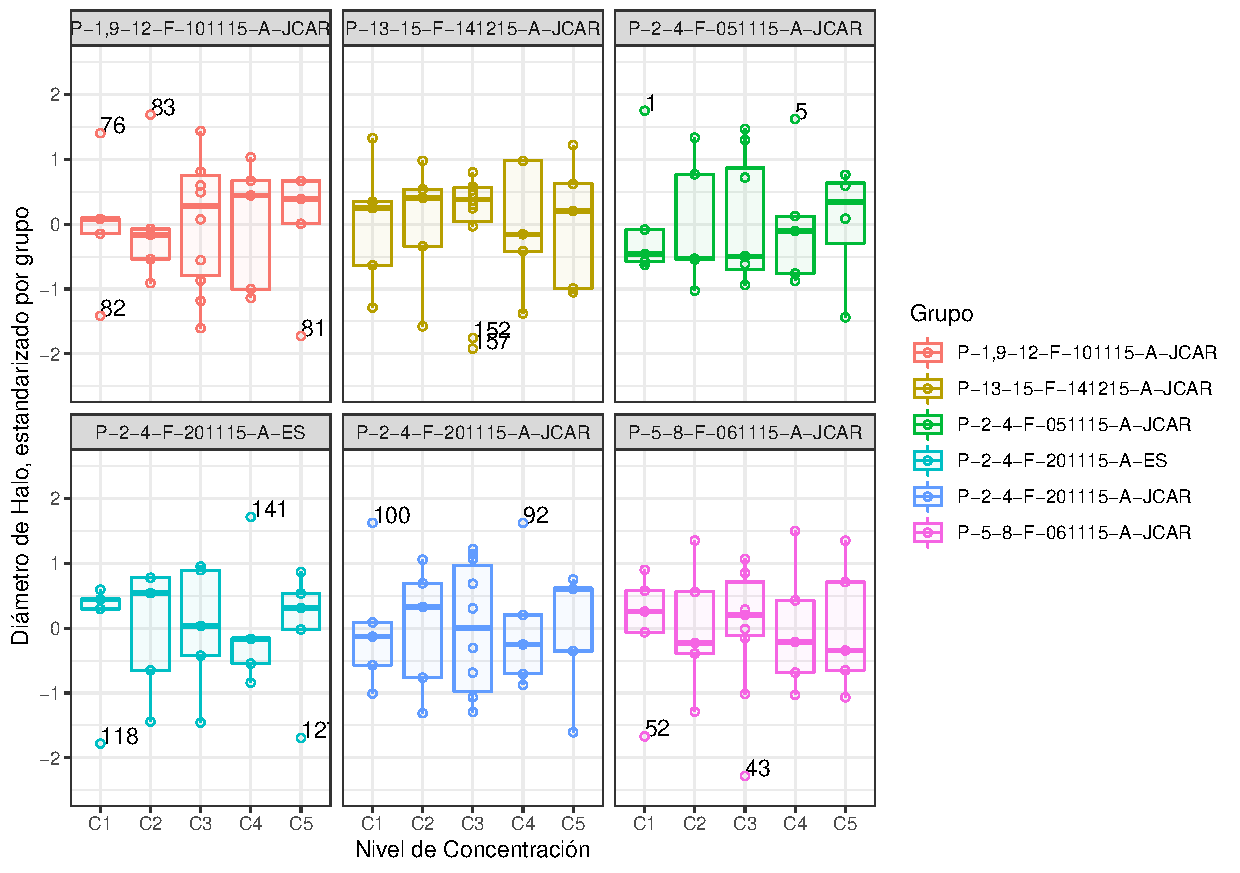
\includegraphics[width=1\linewidth]{Figuras/01_Outliers_identificados.pdf}
	\caption[Se muestran los datos atípicos como aquellos con un rango mayor a 1.5 IQR en su grupo principal]{Análisis de datos atípicos por método univariado.}
	\label{Fig:1}
\end{figure}

Se realizó un análisis de los datos de forma bivariada para encontrar datos atípicos. Se ajustó un modelo de regresión lineal, para ello se tomaron los datos de $\phi$ promedio por subgrupo, y se ajustaron como variable dependiente, frente a logaritmo natural de la concentración nominal ($\ln{\mathrm{C_{nom}}} $) como variable independiente. Con el modelo y los datos originales de $\phi$ se realizó la retropredicción de los datos de concentración $ \mathrm{C_{pred}} $, y estos se graficaron frente a los valores de concentración nominal $\mathrm{C_{nom}}$.\\

\noindent
En la Figura \ref{Fig:2} se puede observar el gráfico de bondad de ajuste con una línea de tendencia central, la curva de cada subgrupo. Se observa que el subgrupo correspondiente a la línea de calibración \textbf{P} 2-4, \textbf{F}: 05 de noviembre de 2015, y \textbf{A}: JCAR no tiene un comportamiento de bondad de ajuste similar al resto, por lo cual se considera como diferente y se recomienda su retiro del análisis. \\

\begin{figure}[h]
	\centering
	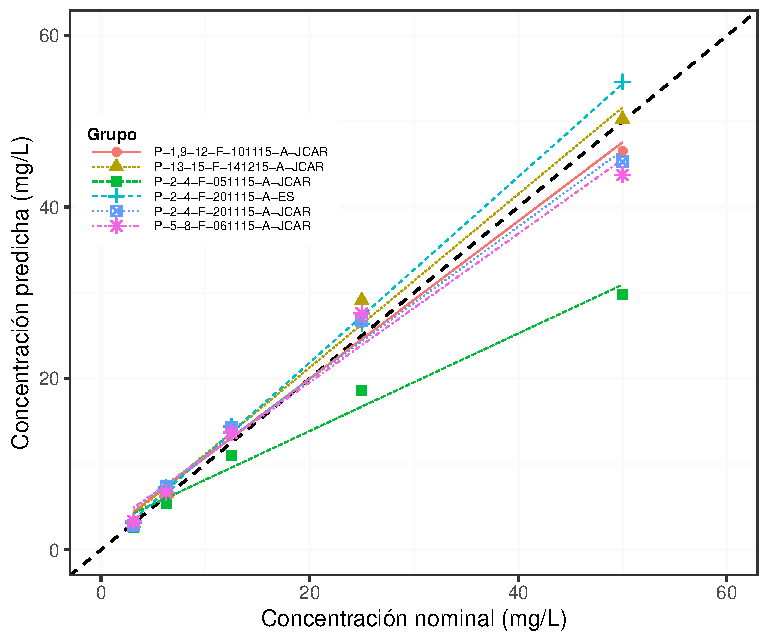
\includegraphics[width=0.8\linewidth]{Figuras/03_Comparacion_CC_1.pdf}
	\caption[Se muestran que una de los subgrupos muestra una desviación importante frente al resto de curvas]{Análisis de bondad de ajuste de análisis de regresión, para curvas de calibración elaboradas.}
	\label{Fig:2}
\end{figure}

Por estas razones se hace su retiro del análisis, y se continua el análisis de la validación sin el mismo. \\

\subsection{Linealidad}
Se cuenta con cinco (5) curvas de calibración con cinco (5) niveles de concentración cada una, se realizó la regresión con diferentes métodos de estimación con y sin ponderación. Los modelos probados fueron: (1) OLS - mínimos cuadrados ordinarios, (2) WLS - mínimos cuadrados ponderados por $\phi^{-1}$, (3) WLS - mínimos cuadrados ponderados por $\phi^{-2}$, (4) WLS - mínimos cuadrados ponderados por $\left(\ln{\mathrm{C_{nom}}}\right)^{-1}$, y (5) WLS - mínimos cuadrados ponderados por $\left(\ln{\mathrm{C_{nom}}}\right)^{-2}$.\\

\noindent
Cada uno de los modelos ensayados describe la siguiente relación: $ \phi = \theta_{0} + \theta_{1}\cdot\ln{\mathrm{C_{nom}}}$, donde $\theta_{0}$ y $\theta_{1} $, son el intercepto y la pendiente de manera respectiva, $ \phi $ es el diámetro del halo de inhibición, y $ \mathrm{C_{nom}} $ es la concentración nominal de cada determinación. En el Cuadro \ref{Cuadro:1} se puede observar un resumen del valor de los parámetros de regresión en la evaluación de modelos. En el cuadro se observa que los modelos presentan valores de parámetros muy similares entre sí, por lo cual se esperan diferencias mínimas en la bondad de ajuste del modelo. \\ 

\begin{table}[H]
	\centering
\begin{tabular}{clcccc}
	\hline
	\multirow{2}{*}{\textbf{Parámetro}}  & \multirow{2}{*}{\textbf{Estimador}}             & \multirow{2}{*}{\textbf{Valor}} & \multirow{2}{*}{\textbf{Error Est.}} & \multirow{2}{*}{\textbf{Valor-t}} & \multirow{2}{*}{$\mathbf{Pr(>|t|)}$} \\
	                                     &                                                 &                                 &                                      &                                   &                                      \\ \hline
	\multirow{5}{*}{\textbf{Intercepto}}  &  OLS                                              & 11.962 & 0.194 & 61.506 & 5.036-27\\
	                                      &  WLS $\phi^{-1}$                                  & 11.850 & 0.183 & 64.638 & 1.617E-27\\
	                                      &  WLS $\phi^{-2}$                                  & 11.746 & 0.173 & 67.71 & 5.587E-28\\
	                                      &  WLS $ \left(\ln{\mathrm{C_{nom}}}\right)^{-1} $  & 11.708 & 0.168 & 69.514 & 3.060E-28\\
	                                      &  WLS $ \left(\ln{\mathrm{C_{nom}}}\right)^{-2} $  & 11.505 & 0.152 & 75.532 & 4.571E-29\\
	\hline
	\multirow{5}{*}{\textbf{Pendiente}}   &  OLS                                              & 3.786 & 0.072 & 52.735 & 1.692E-25\\
	                                      &  WLS $\phi^{-1}$                                  & 3.828 & 0.072 & 53.147 & 1.417E-25\\
	                                      &  WLS $\phi^{-2}$                                  & 3.869 & 0.073 & 52.969 & 1.530E-25\\
	                                      &  WLS $ \left(\ln{\mathrm{C_{nom}}}\right)^{-1} $  & 3.886 & 0.073 & 53.089 & 1.453E-25\\
	                                      &  WLS $ \left(\ln{\mathrm{C_{nom}}}\right)^{-2} $  & 3.983 & 0.08 & 49.655 & 6.677E-25\\
	\hline
\end{tabular} 
\caption{Valor de parámetros de regresión lineal en modelos lineales explorados.}
\label{Cuadro:1}
\end{table}

Se realizó una comparación de parámetros de bondad de ajuste de los modelos probados (ver Cuadro \ref{Cuadro:2}). Todos los modelos cuentan con una bondad de ajuste apropiada, y pasan el test F. Se tiene que el mejor modelo por su valor de estadístico $ \mathrm{F_{calc}} $ es el modelo WLS con ponderación en la variable dependiente ($\phi^{-1}$). Sin embargo, el modelo con menor error residual estándar $\mathrm{RSE}$ es el modelo WLS que tiene ponderación por $\phi^{-2}$. Los modelos con ponderación $\phi^{-1}$ y $\left(\ln{\mathrm{C_{nom}}}\right)^{-1}$ cuentan con un valor de coeficiente de correlación ($ \mathrm{r^{2}_{adj.}} $) similar. Considerando que el valor de $\mathrm{F_{calc}}$ tiene más fundamento desde la probabilidad, se escoge al modelo WLS con ponderación $\phi^{-1}$ como el mejor, dentro de esto conjunto de modelos ensayados.\\

\begin{table}[H]
	\centering
	\begin{tabular}{lccccccc}
		\hline
		\textbf{Estimación} & \textbf{RSE} & \textbf{gL} & $ \mathbf{r^{2}} $ & $ \mathbf{r^{2}_{adj.}} $ & $ \mathbf{F_{calc}} $ & $ \mathbf{F_{tab.}} $ & $ \mathbf{p} $ \\ \hline
		OLS          &    0.3518    &     23      &       0.9918       &          0.9914           &         2781.0          &         248.8         &  1.692E-25  \\
		WLS $\phi^{-1}$          &    0.0774    &     23      &       0.9919       &          0.9916           &        2824.6         &         248.8         &  1.417E-25  \\
		WLS $\phi^{-2}$          &    0.0171    &     23      &       0.9919       &          0.9915           &        2805.7         &         248.8         &  1.530E-25  \\
		WLS $ \left(\ln{\mathrm{C_{nom}}}\right)^{-1} $          &    0.2399    &     23      &       0.9919       &          0.9916           &        2818.4         &         248.8         &  1.453E-25  \\
		WLS $ \left(\ln{\mathrm{C_{nom}}}\right)^{-2} $          &    0.1698    &     23      &       0.9908       &          0.9904           &        2465.6         &         248.8         &  6.677E-25  \\ \hline
	\end{tabular} 
\caption{Parámetros relacionados a la bondad de ajuste de modelos probados.}
\label{Cuadro:2}
\end{table}

\noindent
En la Figura \ref{Fig:3}, se puede observar la curva de calibración con el modelo de elección que es WLS con ponderación de tipo $\phi^{-1}$. Se observa que la mayoría de las observaciones muestran una relación cercana al modelo ajustado, y se observa que existe una tendencia de los puntos a ser curvilíneos en concentraciones mayores. \\


\begin{figure}[H]
	\centering
	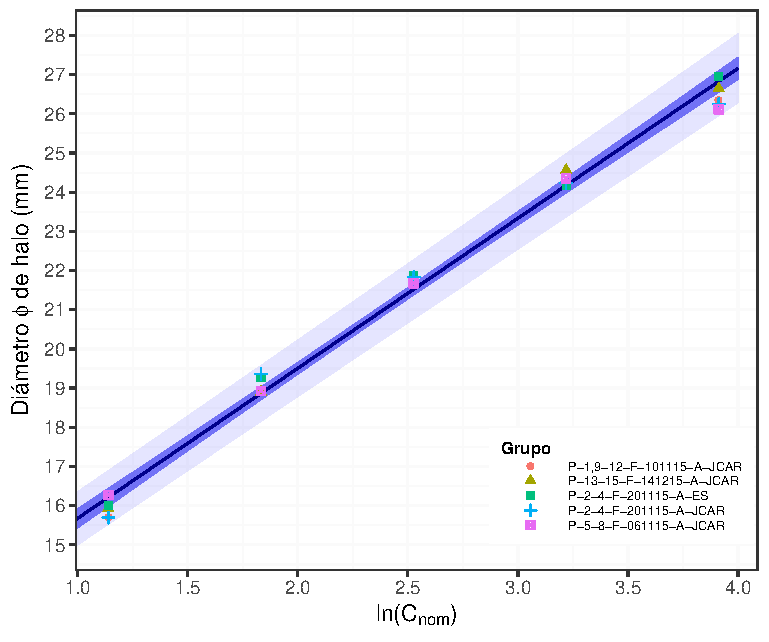
\includegraphics[width=0.8\linewidth]{Figuras/22_curva_calibracion_1.pdf}
	\caption[Diferentes modelos de regresión]{Curva de calibración con modelo de regresión lineal ponderada (WLS) con ponderación de tipo $\phi^{-1}$.}
	\label{Fig:3}
\end{figure}

\noindent
En el Cuadro 3 se observa una resumen de los datos de regresión del modelo escogido, estos coinciden con los mostrado en los cuadros \ref{Cuadro:1}, y \ref{Cuadro:2}. \\

\begin{table}[H]
	\centering
	\begin{tabular}{|llllll|}
		\hline
		
		\multicolumn{6}{|c|}{\multirow{2}{*}{\textbf{Análisis de Regresión - Modelo WLS ($\mathbf{\phi^{-1}}$):  $\mathbf{\phi}=\mathbf{\theta_{0}}$ + $\mathbf{\theta_{1}\cdot}$ $\mathbf{\ln{\mathrm{C_{nom}}}}$}}} \\
		 & & & & & \\
		\hline
		\multicolumn{6}{|l|}{\textbf{Estimación}} \\
		\textbf{Parámetro} & \textbf{Valor} & \textbf{Error Est.} & \textbf{Valor t} & \multicolumn{2}{l|}{\textbf{Valor P}} \\ \hline
		Intercepto & 11.850 & 0.183 & 64.64 & <2E-16 & *** \\ 
		Pendiente & 3.828 & 0.072 & 53.15 & <2E-16 & *** \\
		
		\multicolumn{6}{|l|}{\begin{tabular}[c]{@{}l@{}}
				$H_0$: $\theta_{0} = 0$;~$\theta_{1} = 0$\\ 
				$H_A$: $\theta_{0} \neq 0$;~$\theta_{1} \neq 0$\\ 
		\end{tabular}} \\  
		\multicolumn{3}{|l}{$\theta_{0}$ - IC 95\%: {[}11.471, 12.230{]}} & 
		\multicolumn{3}{l|}{$\theta_{1}$ - IC 95\%: {[}3.679, 3.977{]}} \\ \hline
		\multicolumn{6}{|l|}{\textbf{ANOVA}} \\ 
		\textbf{Fuente} & \textbf{gL} & \textbf{SC} & \textbf{MC} & $\mathbf{F_{calc.}}$ & \textbf{P} \\ \hline
		Pendiente & 1 & 16.90 & 16.90 & 2824.6 & \textless{}2.2E-16 \\ 
		Residuales & 23 & 0.1376 & 0.006 &  &  \\ 
		Total & 24 & 17.0391 &  &  &  \\ \hline
		\multicolumn{6}{|l|}{RSE: 0.07735 con 23gL} \\
		\multicolumn{3}{|l}{$R^{2}$: 0.9919} & \multicolumn{3}{l|}{$R^{2}_{\mathrm{adj}}$: 0.9916}\\ \hline
	\end{tabular}	
	\caption{Resultado de modelo de regresión lineal elegido WLS con ponderación $\mathrm{\phi^{-1}}$ \label{Cuadro:3}}
\end{table}

\noindent
En la Figura \ref{Fig:4} se muestra una comparación entre las concentraciones nominales y retropredichas de los cuatro modelos que muestran resultados muy similares. Se observa que a las concentraciones más altas el método tiende a realizar subestimar las concentraciones, lo cual podría generar un sesgo en la estimación de parámetros farmacocinéticos (p.ej. $\mathrm{V}$). Se deduce que en el rango de concentraciones de $3.125-50\conc$, el método no se encuentra en un rango lineal, pero aún podría ser considerado como rango dinámico. Pese a esto, no se considera realizar un ajuste de las observaciones a un modelo cuadrático debido a que se desconoce el comportamiento real de los datos a concentraciones altas por la falta de determinaciones en esta región. \\

\begin{figure}[ht]
	\centering
	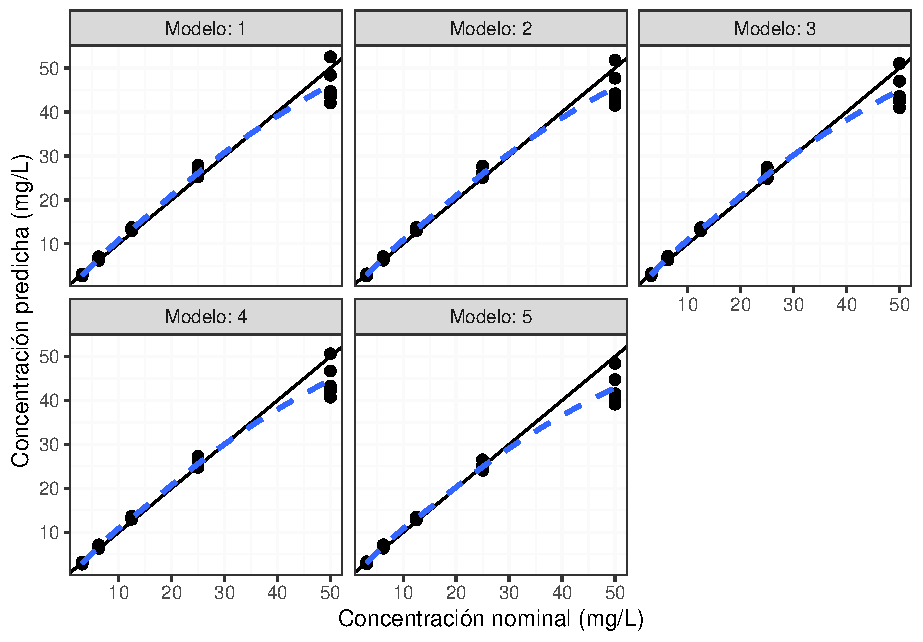
\includegraphics[width=0.8\linewidth]{Figuras/24_Comparacion_CC_2.pdf}
		\caption[Diferentes modelos de regresión]{Análisis de bondad de ajuste de análisis de regresión, con diversos modelos de regresión. Modelo 1: OLS, Modelo 2: WLS $\phi^{-1}$, Modelo 3: WLS $\phi^{-2}$, Modelo 4: $\left(\ln{\mathrm{C_{nom}}}\right)^{-1}$, y Modelo 5: $\left(\ln{\mathrm{C_{nom}}}\right)^{-2}$. En negro se muestra la predicción del modelo, en azul oscuro se muestra el intervalo de confianza alrededor de la curva de calibración, y en un azul más claro se muestra el intervalo de predicción del modelo.}
	\label{Fig:4}
\end{figure}

\noindent
En la Figura \ref{Fig:5} y Figura \ref{Fig:6} se observan gráficos para evaluar la bondad de ajuste del modelo mediante errores residuales relativos ($ \mathrm{ER} $) a la concentración nominal del modelo ($\mathrm{C_{nom}}$). El error residual relativo de cada predicción se calcula mediante la fórmula en la ecuación \ref{Eq:1}: \\

\begin{equation}\label{Eq:1}
	\mathrm{ER}_{i} = \frac{\ln{\mathrm{C_{i}}} - \ln{\mathrm{\hat{C}_{i}}}}{\ln{\mathrm{C_{i}}}} = \frac{\ln{\mathrm{C_{i}}} - \left(\phi_{i} + \theta_{0}\right) / \theta_{1}}{\ln{\mathrm{C_{i}}}}
\end{equation} \\

\noindent
En donde, $ \mathrm{\hat{C}_{i}} $ corresponde a las concentraciones nominales $ \mathrm{C_{nom}} $, mientras que $ \mathrm{\hat{C}_{i}} $ corresponde a las concentraciones retropredichas $ \mathrm{C_{pred}} $. En las Figuras \ref{Fig:5} y \ref{Fig:6} se observa que la varianza permanece relativamente constante, y por tal se cumple el supuesto de homocesdasticidad. Sólo en dos puntos del gráfico los residuales sobrepasan los valores de referencia de $\pm 0.15$ para >LLOQ, y $\pm 0.20$ para LLOQ.\\

\noindent
Por último, se comprobaron supuestos de normalidad de residuales con el test de Shapiro-Wilk ($ W $=0.923, valor $ p $ = 0.060) por lo cual para un $ \alpha = 0.05 $ se puede rechazar la $H_{0}$ de que los residuales provienen de una distribución normal. Para la comprobación de homocesdasticidad se realizó el test de Breusch-Pagan, que tomó un grado de liberta de 1, y $\chi^{2} = 0.245$, y valor $p =0.6203$ que es mayor a 0.05, por lo cual no se puede rechazar la hipótesis nula, lo que implica que no se espera heterocesdasticidad significativa.\\

\begin{info}
	La mayoría de las predicciones no se alejan por más de 15 a 20\% del valor de concentración, y se cumple este criterio para >75\% de las muestras con estándar analizadas. Por el cumplimiento de este criterio se considera que el método es \textbf{lineal}. 
\end{info}

\begin{figure}[H]
	\centering
	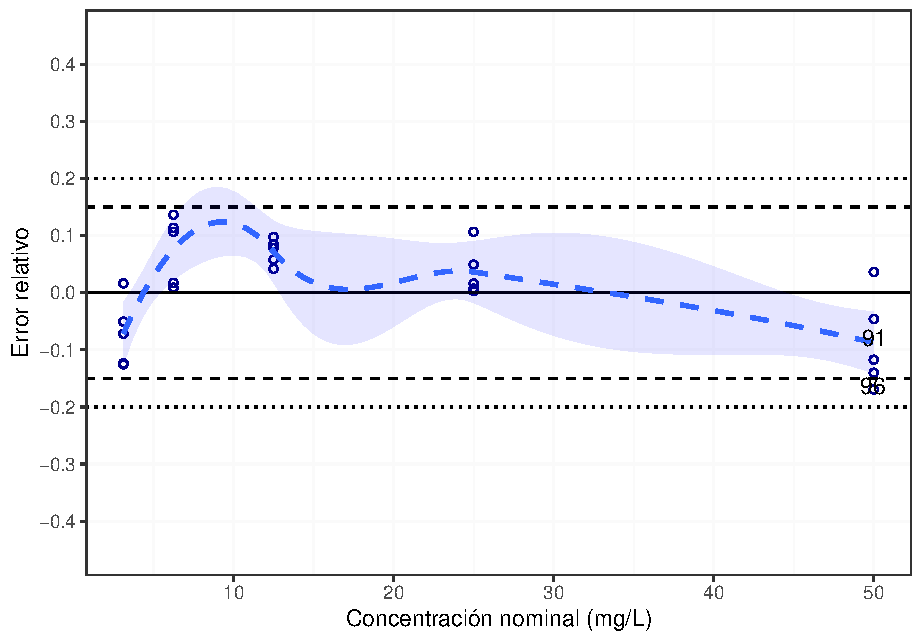
\includegraphics[width=0.8\linewidth]{Figuras/25_Grafico_error_concentracion.pdf}
	\caption[GOF error vs concentración predicha]{Gráfico de bondad de ajuste con $\mathrm{C_{nom}}$ vs error relativo del modelo de regresión.}
	\label{Fig:5}
\end{figure}

\begin{figure}[H]
	\centering
	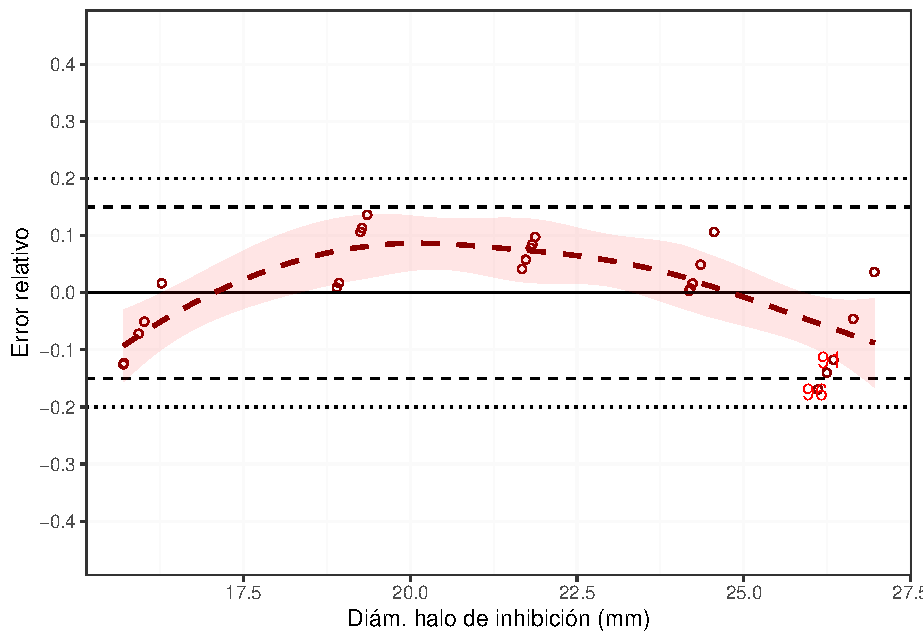
\includegraphics[width=0.8\linewidth]{Figuras/26_Grafico_error_diametro_halo.pdf}
	\caption[GOF error vs diámetro de halo]{Gráfico de bondad de ajuste con $\phi$ de halo de inhibición vs error relativo del modelo de regresión.}
	\label{Fig:6}
\end{figure}


\subsection{Exactitud y Precisión}\label{Exactitud}
Para determinar la exactitud de este método se utilizaron los mismos datos provenientes de la curva de calibración, la exactitud se obtiene al realizar un promedio de los valores de retropredicción ($ \mathrm{\bar{C}}_{\mathrm{pred}} $) y comparando frente a valores de concentración nominal ($ \mathrm{C}_{\mathrm{nom}} $), por cada nivel de concentración. \\

\begin{equation}\label{Eq:2}
	\mathrm{ER} = \frac{\sum_{1}^{n}{\mathrm{C_{pred}}/n - \mathrm{C_{nom}}}}{\mathrm{C_{nom}}}
\end{equation}\\

\noindent
En la Figura \ref{Fig:RSD} se pueden observar los resultados de exactitud (\ref{Fig:RSD_A}) y precisión (\ref{Fig:RSD_B}) para el método. En las figuras se colocaron líneas punteadas en los valores de referencia que no debían ser sobrepasados para la aceptación del método. El punto de calibración con mayor sesgo fue C1 con $ +9\% $ de sesgo, pero esto no supera el límite de $\pm15\% $. Por otra parte, la precisión inter-ensayo se encontró en un rango de $ 2.08-9.07\% $ medido como $ \mathrm{RSD} $. \\

\begin{figure}[h]
	\centering
	\begin{subfigure}[b]{0.49\textwidth}
		\centering
		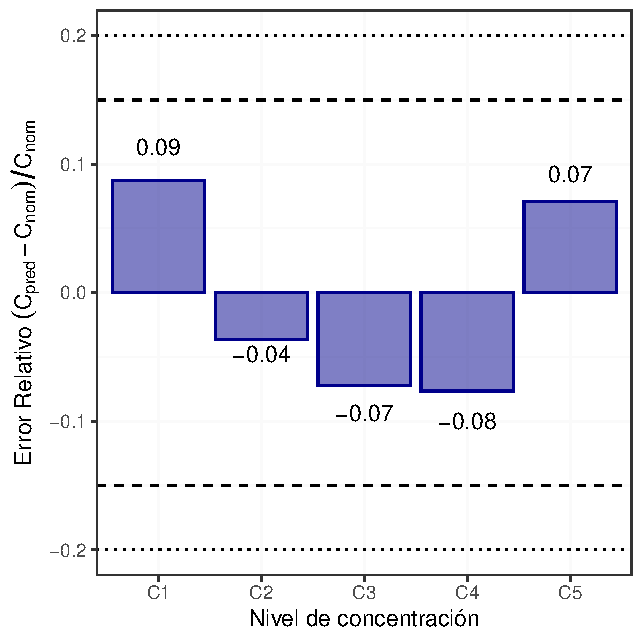
\includegraphics[width=1\linewidth]{Figuras/27_Exactitud_metodo.pdf}
		\caption{Gráfico con error relativo a la concentración nominal de valor medio de concentración predicha.}
		\label{Fig:RSD_A}
	\end{subfigure}
	\hfill
	\begin{subfigure}[b]{0.49\textwidth}
	\centering
	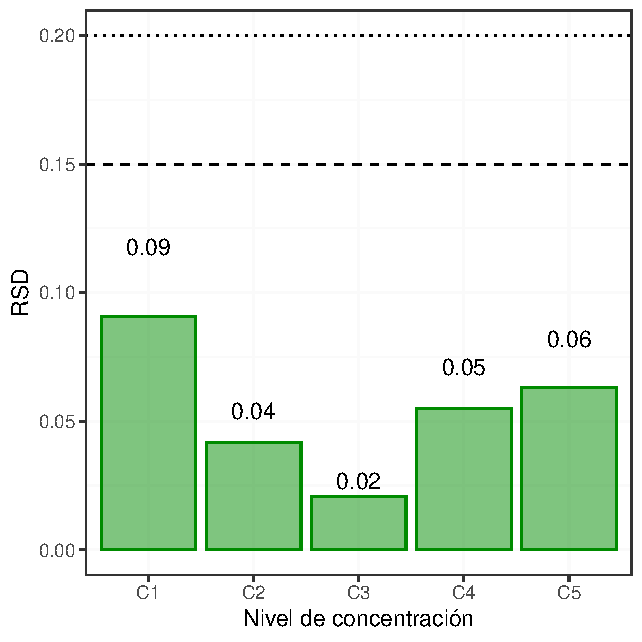
\includegraphics[width=1\linewidth]{Figuras/28_Repetibilidad_metodo.pdf}
	\caption{Gráfico con RSD de $\mathrm{C_{pred}}$ para cada nivel de concentración.}
	\label{Fig:RSD_B}
	\end{subfigure}

	\caption{Parámetros de validación de modelo. Se muestra el criterio de aceptación para muestras mayores a LLOQ con la línea con guiones, y el criterio de aceptación para LLOQ con una línea punteada.}
	\label{Fig:RSD}
\end{figure}

\noindent
La precisión intermedia fue evaluada teniendo en cuenta las repeticiones dentro de cada grupo, que podrían equivaler a lotes analíticos diferentes. No se puede evaluar la precisión para los factores por separado (día, suero inicial, o analista) ya que no existe un diseño balanceado de los factores. Se utilizó un análisis por ANOVA teniendo en cuenta la siguiente tabla de una análisis ANOVA de un factor: \\

\begin{table}[H]
	\centering
\begin{tabular}{llcccc}
	\hline
	%\multirow{2}{*}{
	\multirow{2}{*}{\textbf{Categoría}} & \multirow{2}{*}{$\mathbf{df}$} & \multirow{2}{*}{\textbf{Sum Cuad.}} & \multirow{2}{*}{\textbf{Media Cuad.}} & \multirow{2}{*}{\textbf{Valor F}} & \multirow{2}{*}{\textbf{Pr(>F)}} \\ &  &  &  &  & \\
	\hline
	Entre grupos & k-1 & $\mathrm{SS_{inter}}$ & $\mathrm{MS_{inter}}$ & F & p        \\

	Intra grupos & N-k & $\mathrm{SS_{intra}}$ & $\mathrm{MS_{intra}}$ &  & \\
	Total & N-1 & $\mathrm{SS_{total}}$ &  &  & \\ \hline
\end{tabular}
\caption{Tabla ANOVA representativa.}
\label{Cuadro:4}
\end{table}

\noindent
Para el cálculo de precisión intermedia se deben tener en cuenta los siguientes fórmulas para el cálculo de los factores.\\

\begin{equation}\label{Eq:3}
	\mathrm{S^{2}_{intra}} = \mathrm{MS_{intra}}
\end{equation}

\begin{equation}\label{Eq:4}
\mathrm{RSD_{intra}(\%)} = \frac{\sqrt{\mathrm{S^{2}_{intra}}}}{\bar{\mathrm{X}}}\cdot 100\%
\end{equation}

\begin{equation}\label{Eq:5}
\mathrm{S^{2}_{inter}} = \frac{\mathrm{MS_{inter}}-\mathrm{MS_{intra}}}{n}
\end{equation}

\begin{equation}\label{Eq:6}
\mathrm{RSD_{inter}(\%)} = \frac{\sqrt{\mathrm{S^{2}_{inter}}+\mathrm{S^{2}_{intra}}}}{\bar{\mathrm{X}}}\cdot 100\%
\end{equation}\\

\noindent
En el Cuadro \ref{Cuadro:5} se pueden observar los resultados del cálculo de precisión intermedia. Se encuentra que la precisión intermedia ($\mathrm{RSD_{inter}}$) no supera el valor de referencia de $ +15\% $, con valores en el rango de $4.8-9.5\%$. La repetibilidad ($\mathrm{RSD_{intra}}$) en este análisis no supera los valores de referencia encontrándose en un rango de $4.2-6.7\%$.\\

\begin{table}[H]
	\centering
\begin{tabular}{ccccccc}
	\hline
	\multirow{2}{*}{$\mathbf{C_{nom}}$} & \multirow{2}{*}{$\mathbf{\bar{C}_{pred}}$} & \multirow{2}{*}{$\mathbf{S^{2}_{intra}}$} & \multirow{2}{*}{$\mathbf{RSD_{intra}(\%)}$} & \multirow{2}{*}{$\mathbf{S^{2}_{inter}}$} & \multirow{2}{*}{$\mathbf{RSD_{inter}(\%)}$} & \multirow{2}{*}{\textbf{Pr>F}} \\ 
	 & & & & & & \\ 
	 \hline
	3.125              &           2.91            &          0.032           &           5.8\%            &          0.028           &           7.9\%            &     0.004     \\

	6.25               &           6.74            &          0.177           &           6.7\%            &          0.103           &           8.5\%            &     0.016     \\
	12.5               &           13.4            &          0.326           &           4.6\%            &          0.029           &           4.8\%            &     0.13      \\
	25                 &           25.9            &          1.123           &           4.2\%            &           0.97           &           5.8\%            &     0.004     \\
	50                 &           45.7            &          6.311           &           5.0\%            &          16.251          &           9.5\%            &    0.00001    \\ \hline
\end{tabular} 
\caption{Resultado de Análisis de Varianza (ANOVA) de un factor.}
\label{Cuadro:5}
\end{table}

\begin{info}
	Se encuentra que las concentraciones retro-predichas cumplen con los criterios de exactitud (error relativo < $\pm 15\%$, y $\pm 20\% $ para LLOQ), repetibilidad (RSD $\textless15\% $, y $\textless20\%$ para LLOQ), y precisión intermedia (RSD $\textless15\% $, y $\textless20\%$ para LLOQ).
\end{info}

\subsection{Límite de cuantificación}
El límite de cuantificación se puede calcular mediante la siguiente ecuación:

\begin{equation}\label{Eq:7}
	\mathrm{LOQ} = 10\cdot c(\mathrm{LOQ})
\end{equation}

\begin{equation}\label{Eq:8}
\mathrm{LOQ} = 10\cdot \frac{\hat{\sigma_{y_0}}}{b}
\end{equation}

\noindent
En el primer caso, $c(\mathrm{LOQ})$ es la mitad del intervalo de confianza en el límite. Con el primer método se tiene un $ \mathrm{LOQ} $ estimado de $1.313\conc $, y con el segundo método  se tiene $1.614\conc$. Si bien se encontraron estos valores estimados, estos no fueron confirmados de manera experimental, por tal se considera a $3.125\conc$.


\section*{Bibliografía}
\bibliography{referencias}


\end{document}

	